\documentclass{ximera}

 

\usepackage{epsfig}

\graphicspath{
  {./}
  {figures/}
}

\usepackage{morewrites}
\makeatletter
\newcommand\subfile[1]{%
\renewcommand{\input}[1]{}%
\begingroup\skip@preamble\otherinput{#1}\endgroup\par\vspace{\topsep}
\let\input\otherinput}
\makeatother

\newcommand{\includeexercises}{\directlua{dofile("/home/jim/linearAlgebra/laode/exercises.lua")}}

%\newcounter{ccounter}
%\setcounter{ccounter}{1}
%\newcommand{\Chapter}[1]{\setcounter{chapter}{\arabic{ccounter}}\chapter{#1}\addtocounter{ccounter}{1}}

%\newcommand{\section}[1]{\section{#1}\setcounter{thm}{0}\setcounter{equation}{0}}

%\renewcommand{\theequation}{\arabic{chapter}.\arabic{section}.\arabic{equation}}
%\renewcommand{\thefigure}{\arabic{chapter}.\arabic{figure}}
%\renewcommand{\thetable}{\arabic{chapter}.\arabic{table}}

%\newcommand{\Sec}[2]{\section{#1}\markright{\arabic{ccounter}.\arabic{section}.#2}\setcounter{equation}{0}\setcounter{thm}{0}\setcounter{figure}{0}}

\newcommand{\Sec}[2]{\section{#1}}

\setcounter{secnumdepth}{2}
%\setcounter{secnumdepth}{1} 

%\newcounter{THM}
%\renewcommand{\theTHM}{\arabic{chapter}.\arabic{section}}

\newcommand{\trademark}{{R\!\!\!\!\!\bigcirc}}
%\newtheorem{exercise}{}

\newcommand{\dfield}{{\sf dfield9}}
\newcommand{\pplane}{{\sf pplane9}}

\newcommand{\EXER}{\section*{Exercises}}%\vspace*{0.2in}\hrule\small\setcounter{exercise}{0}}
\newcommand{\CEXER}{}%\vspace{0.08in}\begin{center}Computer Exercises\end{center}}
\newcommand{\TEXER}{} %\vspace{0.08in}\begin{center}Hand Exercises\end{center}}
\newcommand{\AEXER}{} %\vspace{0.08in}\begin{center}Hand Exercises\end{center}}

% BADBAD: \newcommand{\Bbb}{\bf}

\newcommand{\R}{\mbox{$\Bbb{R}$}}
\newcommand{\C}{\mbox{$\Bbb{C}$}}
\newcommand{\Z}{\mbox{$\Bbb{Z}$}}
\newcommand{\N}{\mbox{$\Bbb{N}$}}
\newcommand{\D}{\mbox{{\bf D}}}
\usepackage{amssymb}
%\newcommand{\qed}{\hfill\mbox{\raggedright$\square$} \vspace{1ex}}
%\newcommand{\proof}{\noindent {\bf Proof:} \hspace{0.1in}}

\newcommand{\setmin}{\;\mbox{--}\;}
\newcommand{\Matlab}{{M\small{AT\-LAB}} }
\newcommand{\Matlabp}{{M\small{AT\-LAB}}}
\newcommand{\computer}{\Matlab Instructions}
\newcommand{\half}{\mbox{$\frac{1}{2}$}}
\newcommand{\compose}{\raisebox{.15ex}{\mbox{{\scriptsize$\circ$}}}}
\newcommand{\AND}{\quad\mbox{and}\quad}
\newcommand{\vect}[2]{\left(\begin{array}{c} #1_1 \\ \vdots \\
 #1_{#2}\end{array}\right)}
\newcommand{\mattwo}[4]{\left(\begin{array}{rr} #1 & #2\\ #3
&#4\end{array}\right)}
\newcommand{\mattwoc}[4]{\left(\begin{array}{cc} #1 & #2\\ #3
&#4\end{array}\right)}
\newcommand{\vectwo}[2]{\left(\begin{array}{r} #1 \\ #2\end{array}\right)}
\newcommand{\vectwoc}[2]{\left(\begin{array}{c} #1 \\ #2\end{array}\right)}

\newcommand{\ignore}[1]{}


\newcommand{\inv}{^{-1}}
\newcommand{\CC}{{\cal C}}
\newcommand{\CCone}{\CC^1}
\newcommand{\Span}{{\rm span}}
\newcommand{\rank}{{\rm rank}}
\newcommand{\trace}{{\rm tr}}
\newcommand{\RE}{{\rm Re}}
\newcommand{\IM}{{\rm Im}}
\newcommand{\nulls}{{\rm null\;space}}

\newcommand{\dps}{\displaystyle}
\newcommand{\arraystart}{\renewcommand{\arraystretch}{1.8}}
\newcommand{\arrayfinish}{\renewcommand{\arraystretch}{1.2}}
\newcommand{\Start}[1]{\vspace{0.08in}\noindent {\bf Section~\ref{#1}}}
\newcommand{\exer}[1]{\noindent {\bf \ref{#1}}}
\newcommand{\ans}{}
\newcommand{\matthree}[9]{\left(\begin{array}{rrr} #1 & #2 & #3 \\ #4 & #5 & #6
\\ #7 & #8 & #9\end{array}\right)}
\newcommand{\cvectwo}[2]{\left(\begin{array}{c} #1 \\ #2\end{array}\right)}
\newcommand{\cmatthree}[9]{\left(\begin{array}{ccc} #1 & #2 & #3 \\ #4 & #5 &
#6 \\ #7 & #8 & #9\end{array}\right)}
\newcommand{\vecthree}[3]{\left(\begin{array}{r} #1 \\ #2 \\
#3\end{array}\right)}
\newcommand{\cvecthree}[3]{\left(\begin{array}{c} #1 \\ #2 \\
#3\end{array}\right)}
\newcommand{\cmattwo}[4]{\left(\begin{array}{cc} #1 & #2\\ #3
&#4\end{array}\right)}

\newcommand{\Matrix}[1]{\ensuremath{\left(\begin{array}{rrrrrrrrrrrrrrrrrr} #1 \end{array}\right)}}

\newcommand{\Matrixc}[1]{\ensuremath{\left(\begin{array}{cccccccccccc} #1 \end{array}\right)}}



\renewcommand{\labelenumi}{\theenumi)}
\newenvironment{enumeratea}%
{\begingroup
 \renewcommand{\theenumi}{\alph{enumi}}
 \renewcommand{\labelenumi}{(\theenumi)}
 \begin{enumerate}}
 {\end{enumerate}\endgroup}



\newcounter{help}
\renewcommand{\thehelp}{\thesection.\arabic{equation}}

%\newenvironment{equation*}%
%{\renewcommand\endequation{\eqno (\theequation)* $$}%
%   \begin{equation}}%
%   {\end{equation}\renewcommand\endequation{\eqno \@eqnnum
%$$\global\@ignoretrue}}

%\input{psfig.tex}

\author{Martin Golubitsky and Michael Dellnitz}

%\newenvironment{matlabEquation}%
%{\renewcommand\endequation{\eqno (\theequation*) $$}%
%   \begin{equation}}%
%   {\end{equation}\renewcommand\endequation{\eqno \@eqnnum
% $$\global\@ignoretrue}}

\newcommand{\soln}{\textbf{Solution:} }
\newcommand{\exercap}[1]{\centerline{Figure~\ref{#1}}}
\newcommand{\exercaptwo}[1]{\centerline{Figure~\ref{#1}a\hspace{2.1in}
Figure~\ref{#1}b}}
\newcommand{\exercapthree}[1]{\centerline{Figure~\ref{#1}a\hspace{1.2in}
Figure~\ref{#1}b\hspace{1.2in}Figure~\ref{#1}c}}
\newcommand{\para}{\hspace{0.4in}}

\renewenvironment{solution}{\suppress}{\endsuppress}

\ifxake
\newenvironment{matlabEquation}{\begin{equation}}{\end{equation}}
\else
\newenvironment{matlabEquation}%
{\let\oldtheequation\theequation\renewcommand{\theequation}{\oldtheequation*}\begin{equation}}%
  {\end{equation}\let\theequation\oldtheequation}
\fi

\makeatother


\title{Equilibria and Linearization}

\begin{document}
\begin{abstract}
\end{abstract}
\maketitle

 \label{S:linearization}
\index{equilibrium}  \index{linearization}

Recall that equilibrium solutions of \eqref{e:nonlinear2}
are found by solving simultaneously the algebraic equations
\begin{equation}
\begin{array}{rcl} 
f(x,y) & = & 0 \\
g(x,y) & = & 0.
\end{array}
\end{equation}
In general, it is a difficult task to solve these algebraic
equations explicitly, except in the simplest of cases. One
example where an explicit solution may be found is
\eqref{e:globalexam}.  In that example, equilibria satisfy
\[
y  =  0 \AND x(2.2+x) = 0.
\]
Thus, there are two equilibria $Z_1=(0,0)$ and $Z_2=(-2.2,0)$
and these equilibria can be seen in Figure~\ref{F:globalb}.  We
know from our earlier discussion that the origin $Z_1$ is a
saddle point --- but what about the other equilibrium $Z_2$?
From the figure, it appears to be a spiral sink --- dynamics
that we associate with complex eigenvalues with negative real
parts.  See Table~\ref{T:hyperbolic} in Section~\ref{S:PlanarSystems}.  
In this section we discuss how we can apply linear theory to 
nonlinear equations. 

Let $F:\R^2\to\R^2$ be the nonlinear mapping 
\[
F(x,y)=(f(x,y),g(x,y)).
\]
\begin{definition}  \label{D:Jacobian}
The {\em Jacobian matrix} \index{matrix!Jacobian}
\index{matrix!Jacobian} of $F$ at the point 
$(x,y)$ is the $2\times 2$ matrix 
\begin{equation}  \label{e:jacobian}
(dF)_{(x,y)} = \mattwo{f_x(x,y)}{f_y(x,y)}{g_x(x,y)}{g_y(x,y)}
\end{equation}
where the subscript denotes partial differentiation.  For example, 
$f_x=\frac{\partial f}{\partial x}$.
\end{definition}

Near an equilibrium, the Jacobian matrix is the best {\em linear\/}
approximation\index{linear!approximation} to the mapping $F$.  
This statement can be formalized using 
Taylor series methods in two variables, but we just accept this fact here. 
\begin{definition}  \label{D:hyperbolic}
An equilibrium is {\em hyperbolic\/} if the eigenvalues of the 
Jacobian matrix have nonzero real part. 
\end{definition} \index{hyperbolic}\index{equilibrium!hyperbolic}

Note that it is easy to compute the Jacobian matrix for linear 
systems.  Indeed, for the linear differential equation
\begin{eqnarray*}
\dot{x} & = & ax+by \\ \dot{y} & = & cx+dy,
\end{eqnarray*}
the Jacobian matrix is just \index{matrix!Jacobian}
\[
(dF)_{(x,y)} = \mattwo{a}{b}{c}{d}
\]
and is independent of $x$ and $y$.  So, not surprisingly, the 
best linear approximation to a linear system is itself.

\begin{theorem} \label{T:linearization} \index{linearization}
Suppose that the system of differential equations
\eqref{e:nonlinear2} has a hyperbolic equilibrium at
$Z_0=(x_0,y_0)$.  Then, on a sufficiently small neighborhood of
$Z_0$, the phase plane for \eqref{e:nonlinear2} is the {\em
same\/} as the phase plane\index{phase!plane} of the system of 
linear differential equations
\begin{equation}  \label{e:linearizedeqn}
\vectwo{\dot{x}}{\dot{y}} = (dF)_{Z_0} \vectwo{x}{y}.
\end{equation}
\end{theorem}  \index{hyperbolic}\index{equilibrium!hyperbolic}
It is difficult to define precisely what we mean by the word
{\em same\/}. Roughly speaking, {\em same\/} means that near 
$Z_0$ there is a nonlinear change of coordinates that 
transforms the nonlinear equation into the linear one.

For example, the Jacobian matrix of \eqref{e:globalexam} at the
equilibrium $Z_2=(-2.2,0)$ is 
\[
(dF)_{Z_2} = \left.\mattwoc{0}{1}{2.2+2x+y}{2.1+x}\right|_{(x,y)=(-2.2,0)} 
= \mattwo{0}{1}{-2.2}{-0.1}.
\]
At the equilibrium $Z_2$ we may use \Matlab to show that the 
eigenvalues of $(dF)_{Z_2}$ are $-0.05\pm 1.4824i$, thus verifying 
that the equilibrium $Z_2$ is a spiral sink. \index{sink} 
It is instructive to use {\pplane}\index{\computer!pplane8} to 
show the phase plane of 
the linearized system\index{linearization}.  
(To show the linearization, click on the 
{\sf Find an equilibrium point} button under the {\sf solutions} 
button.  Then in the {\sf PPLANE8 equilibrium point} window click 
on the {\sf display the linearization} button.)  The result is
shown in Figure~\ref{F:spiral} (left); compare this result 
with the phase plane picture in Figure~\ref{F:globalb} (left) 
near the spiral sink.

\begin{figure*}[htb]
           \centerline{%
	   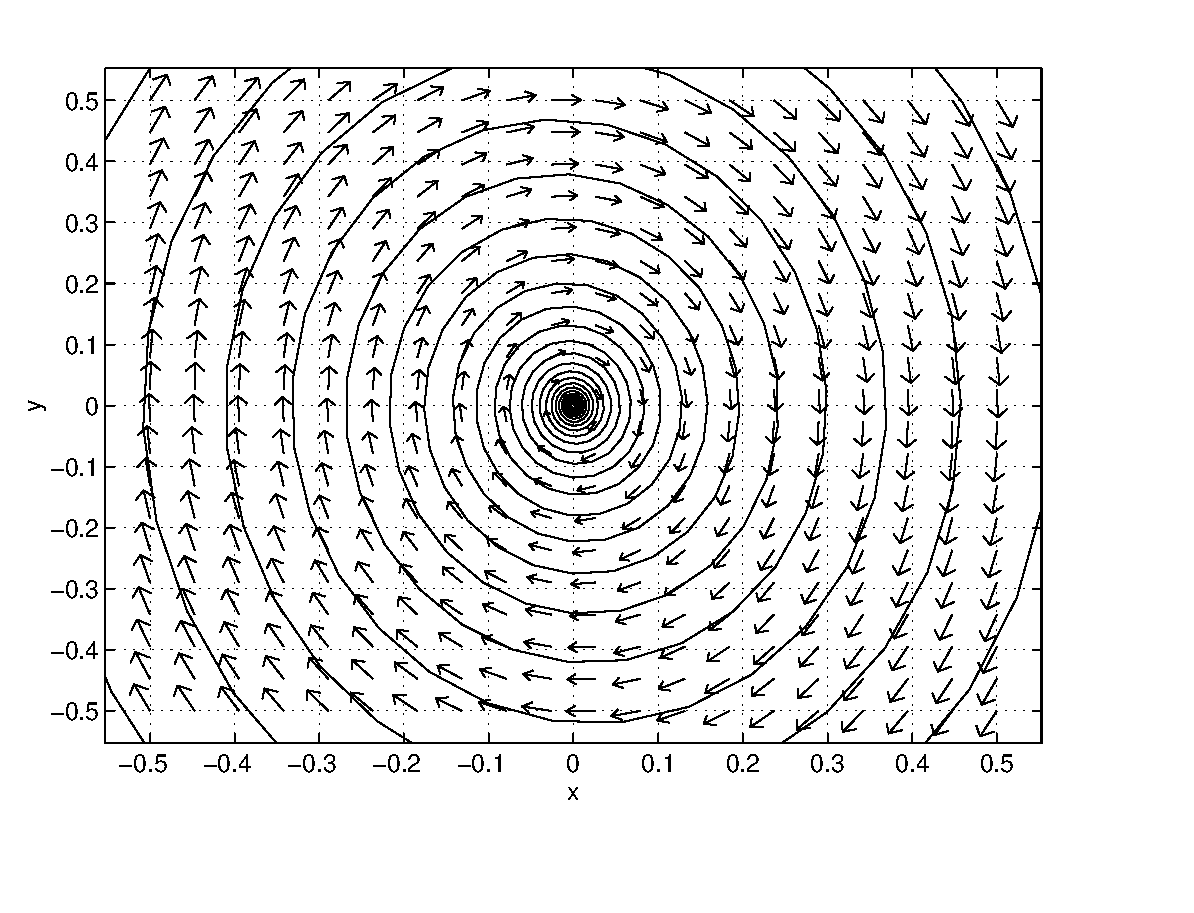
\psfig{file=../figures/spirala.eps,width=3.5in}
           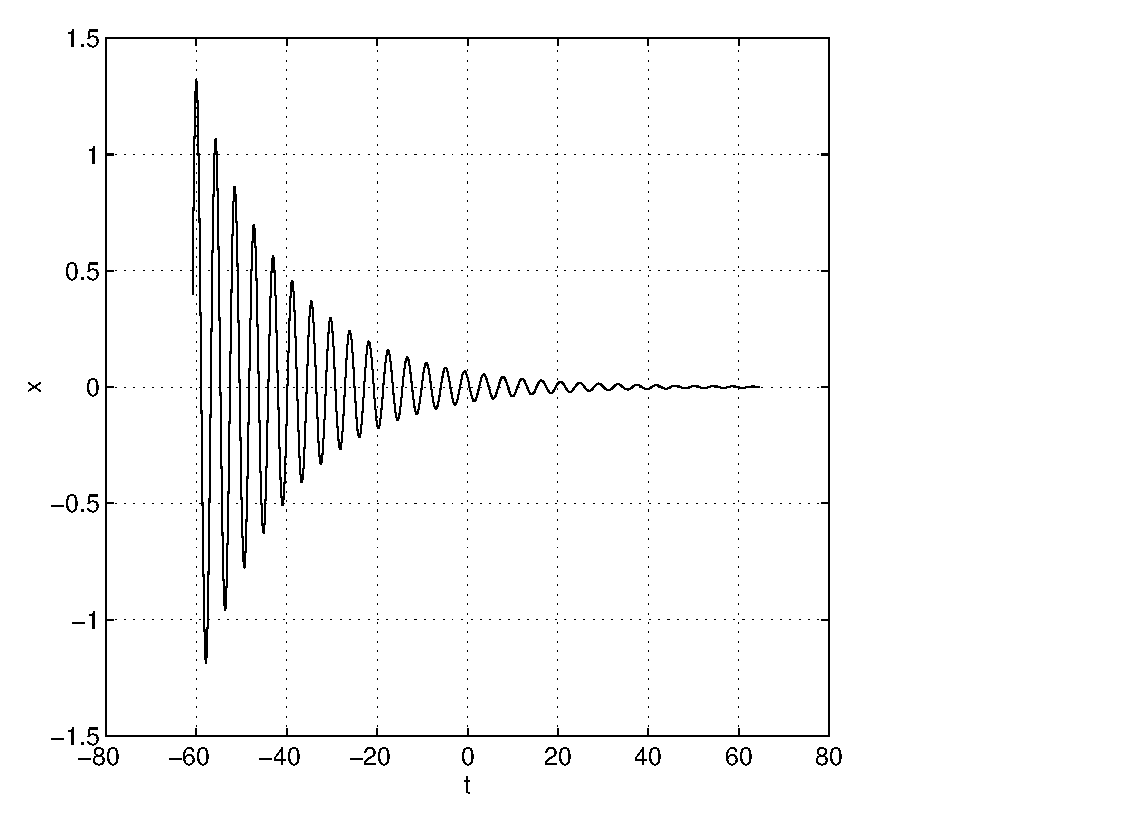
\psfig{file=../figures/spiralb.eps,width=3.0in}}
           \caption{(Left) Trajectory of \protect\eqref{e:linearizedeqn} 
	     near the spiral sink $Z_2$. (Right) The time series $x$ 
		versus $t$ for this solution.}
           \label{F:spiral}
\end{figure*}


There is an important corollary to Theorem~\ref{T:linearization}.
We say that an equilibrium is 
{\em linearly stable\/}\index{stability!linear}
if all of the eigenvalues of the Jacobian matrix have negative real part.

\begin{corollary} \label{C:linearstability}
An equilibrium that is linearly stable is asymptotically stable.
\end{corollary}  \index{stability!asymptotic} 

In Section~\ref{S:PlanarSystems} we discussed linear stability
of the origin for planar linear equations.  We showed (see
Theorem~\ref{T:linstab}) that in planar linear equations, linear
stability implies that the origin is asymptotically stable.  It
follows from Theorem~\ref{T:linearization} that the equilibrium
of the nonlinear equation is also asymptotically stable.  

\begin{remark} 
Generalizations of Theorem~\ref{T:linearization} and 
Corollary~\ref{C:linearstability} to $n$ dimensions are both valid. 
{\rm The Jacobian matrix -- the matrix of partial 
derivatives of the coordinate functions --- is now an $n\times n$
matrix.  In $n$ dimensions, {\em hyperbolicity\/} 
of an equilibrium means that no eigenvalue of the Jacobian matrix has 
zero real part, and {\em linear stability\/} of an equilibrium means 
that the real parts of all $n$ of the eigenvalues have negative real 
part.  See Chapter~\ref{C:HDS}, Theorem~\ref{T:linstab}.}
\end{remark} \index{hyperbolic} \index{matrix!Jacobian}

\subsection*{Important Features of Hyperbolic Equilibria}
\index{equilibrium!hyperbolic}

Theorem~\ref{T:linearization} states that a nonlinear autonomous
system of differential equations behaves like its linearization 
in a small neighborhood of a hyperbolic equilibrium.  To effectively
utilize this theorem, we need to know the important features of phase 
portraits for hyperbolic linear systems.  We now recall results of 
Section~\ref{S:PlanarSystems}.

\subsubsection*{Saddles}  \index{saddle}

Recall from Section~\ref{S:6.7} (see Definition~\ref{D:stablemfld})
that planar systems of linear differential equations with saddles at the 
origin have invariant lines (or eigendirections) called stable and unstable 
orbits.  One eigendirection corresponds to a negative eigenvalue and is 
the stable direction\index{stable!direction}, as solutions on that line 
tend to the origin in forward time.
The other eigendirection corresponds to a positive eigenvalue 
and is the unstable direction\index{unstable!direction}, as solutions on 
that line tend to the origin in backward time.

It follows from Theorem~\ref{T:linearization} that this structure is
approximately recreated in nonlinear systems on small neighborhoods of
saddles.  In particular, there are invariant curves for nonlinear systems 
defined near saddle equilibria.  The nonlinearities deform the invariant 
lines into invariant curves called {\em invariant manifolds\/}.  
\index{stable!manifold} \index{unstable!manifold}  These invariant manifolds 
are called {\em stable\/} and {\em unstable manifolds\/} or {\em stable\/} 
and {\em unstable orbits\/}\index{stable!orbit} \index{unstable!orbit}; 
stable orbits tend to the equilibrium in forward 
time and unstable orbits tend to the equilibrium in backward time.  See 
Figure~\ref{F:globalb} for an example. 

\subsubsection*{Sinks}   \index{sink}

In \eqref{e:globalexam} we have also seen that the spiraling behavior near a
spiral equilibrium is unaffected by higher order terms (see
Figure~\ref{F:globalb}); this remark is also a consequence of
Theorem~\ref{T:linearization}. Similarly, Theorem~\ref{T:linearization} 
guarantees that near an improper node\index{improper node} or a 
focus\index{focus}, higher order terms do not 
affect the local phase portrait of the nonlinear system.

\subsubsection*{An Example with Analytically Solvable Equilibria}

As an example, consider the system of ODEs
\arraystart
\begin{matlabEquation} \label{e1:exer}
\begin{array}{crcl}
(a) & \dps\frac{dx}{dt} & = & 1 + x - y^2  \\
(b) & \dps\frac{dy}{dt} & = & -1 +6y + x^2 - 5y^2 
\end{array}
\end{matlabEquation}
\arrayfinish
We find all of the equilibria of this system of differential
equations, and their type.  (The coefficients have been chosen
so that the calculations are feasible.  Nevertheless, it is
instructive to verify the details.)

Note that $x=y^2-1$ is the solution to \eqref{e1:exer}(a), which we
may substitute into \eqref{e1:exer}(b) to obtain
\[
y^4 - 7y^2 + 6y =0.
\]
The coefficients were chosen so that this polynomial factors
into 
\[
y(y-1)(y-2)(y+3) = 0.
\]
Thus there are four equilibria\index{equilibrium} and they are:
\[
(-1,0),\; (0,1),\; (3,2),\; (8,-3).
\]

We now determine the type of each equilibrium.  To do this,
observe that the Jacobian matrix\index{matrix!Jacobian} 
is:
\[
\left(\begin{array}{cc} 1 & -2y \\ 2x & 6-10y
\end{array}\right). 
\]
Evaluating the Jacobian matrix at the four equilibria, we obtain
\[
\mattwo{1}{0}{-2}{6}, \quad \mattwo{1}{-2}{0}{-4}, \quad
\mattwo{1}{-4}{6}{-14}, \quad \mattwo{1}{6}{16}{36}.
\]
The determinant\index{determinant}, trace\index{trace}, 
discriminant\index{discriminant}, and type of each of these
matrices is shown in Table~\ref{t:exertype}.
\begin{table}[htb]
\begin{center}
\begin{tabular}{|c|c|c|c|c|}
\hline
equilibria & det (d) & trace (t) & disc (D) & type \\
\hline
$(-1,0)$ & $6$ & $7$ & $25$ & nodal source \\
\hline
$(0,1)$ & $-4$ & --- & --- & saddle \\
\hline
$(3,2)$ & $10$ & $-13$ & 129 & nodal sink \\
\hline
$(8,-3)$ & $-60$ & --- & --- & saddle\\
\hline
\end{tabular}
\caption{Types of equilibria in Example~\protect\eqref{e1:exer}.}
\label{t:exertype}
\end{center}
\end{table}\index{nodal source}\index{saddle}\index{nodal sink}

Next we use the information about equilibria contained in 
Table~\ref{t:exertype} and {\pplane}
\index{\computer!pplane8} to compute numerically the 
phase portrait\index{phase!portrait} of equations \eqref{e1:exer}.  Using 
the {\sf Find the equilibrium} button, put circles around
the four equilibria.  (Remember to make the display screen large
enough --- say $-2\leq x \leq 10$ and $-4\leq y \leq 4$.) Also
let {\pplane} compute the stable and unstable orbits of
the two saddles, obtaining the picture in Figure~\ref{F:ex12}.
Once this picture is drawn we have a good idea of the phase
portrait --- note, in particular, the saddle sink and saddle
source connections.


\begin{figure}[htb]
           \centerline{%
           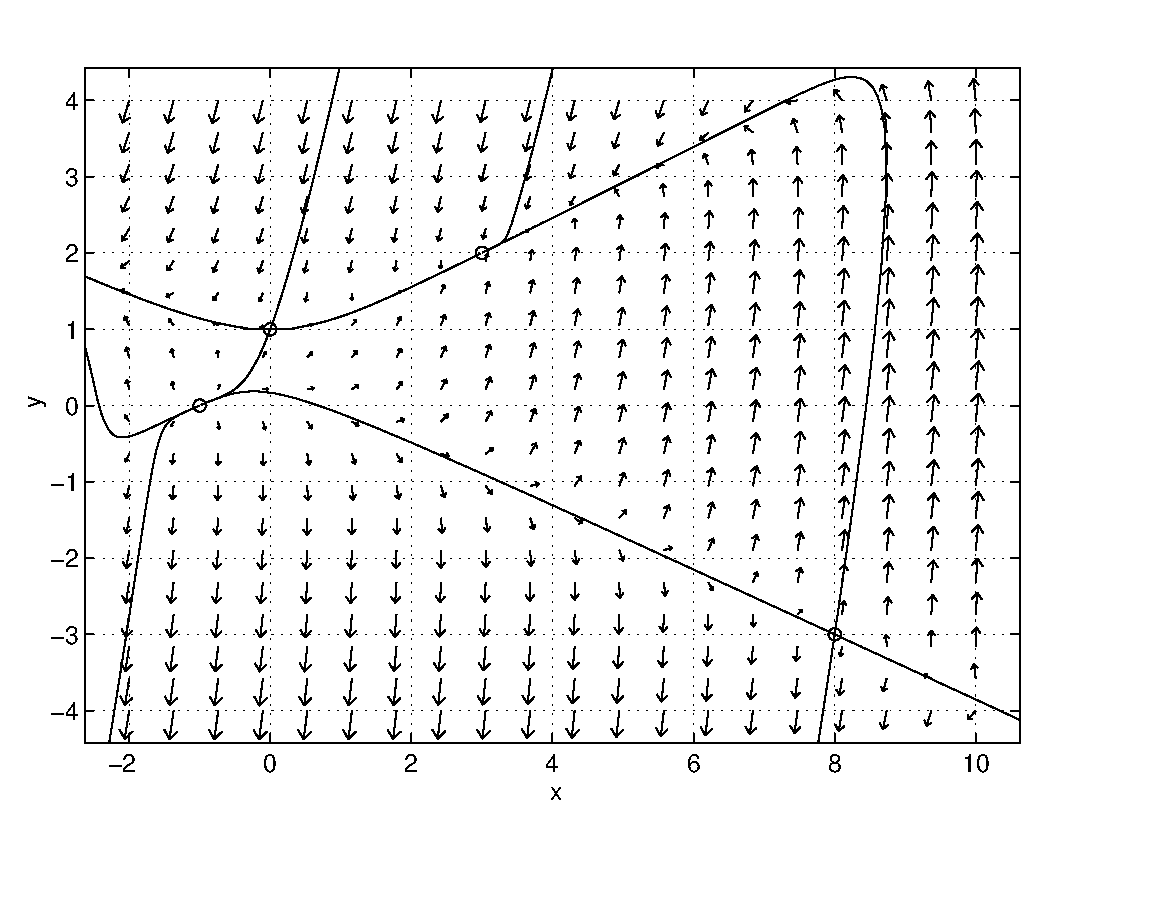
\psfig{file=../figures/ex12exam.eps,width=3.5in}}
		\caption{Equilibria and connections of \protect\eqref{e1:exer}.} 
           \label{F:ex12}
\end{figure}

\subsubsection*{An Example Where Equilibria are Not Analytically Solvable}

As a second example consider the system of differential
equations
\begin{matlabEquation} \label{e:gradexam}
\begin{array}{rcl}
\dot{x} & = & x + y + x^2 - y^2 + 0.1 \\
\dot{y} & = & y - 2xy + 0.5x^2 + y^2.
\end{array}
\end{matlabEquation}
It is difficult to find the equilibria in \eqref{e:gradexam} explicitly.
We can, however, construct the phase plane of this equation with the 
help of {\pplane}.  First we choose a square in which to display 
the direction field\index{direction field} --- say $-5\leq x,y \leq 5$. See 
Figure~\ref{F:gradexam} (left).  We then inspect the direction field 
for possible equilibria.  There is one equilibrium near the origin;  
when we use the {\pplane} search feature for equilibria by clicking 
on the origin, we find a spiral source. Similarly, using the search feature 
for equilibria by clicking along the negative $x$ axis leads to a saddle.  
Once a saddle is found, instructing {\pplane} to plot the stable and 
unstable orbits of this saddle helps to fill in the phase plane.  
Some experimentation yields the four equilibria and connecting stable 
and unstable orbits pictured on the right in Figure~\ref{F:gradexam}.
These equilibria, which are listed by {\pplane} using the {\sf List
computed equilibrium points} button, are:
\begin{verbatim}  
(-0.1066, -0.0047)      Spiral source.           
(-1.1368, -0.2110)      Saddle point.            
(3.2539, 4.2672)        Saddle point.            
(0.2752, -0.3372)       Saddle point.       
\end{verbatim}
It is this last picture that leads to the stylized phase plane portrait 
in Figure~\ref{F:gradexamstyle}. \index{stylized phase portrait}

\begin{figure*}[htb]
           \centerline{%
	   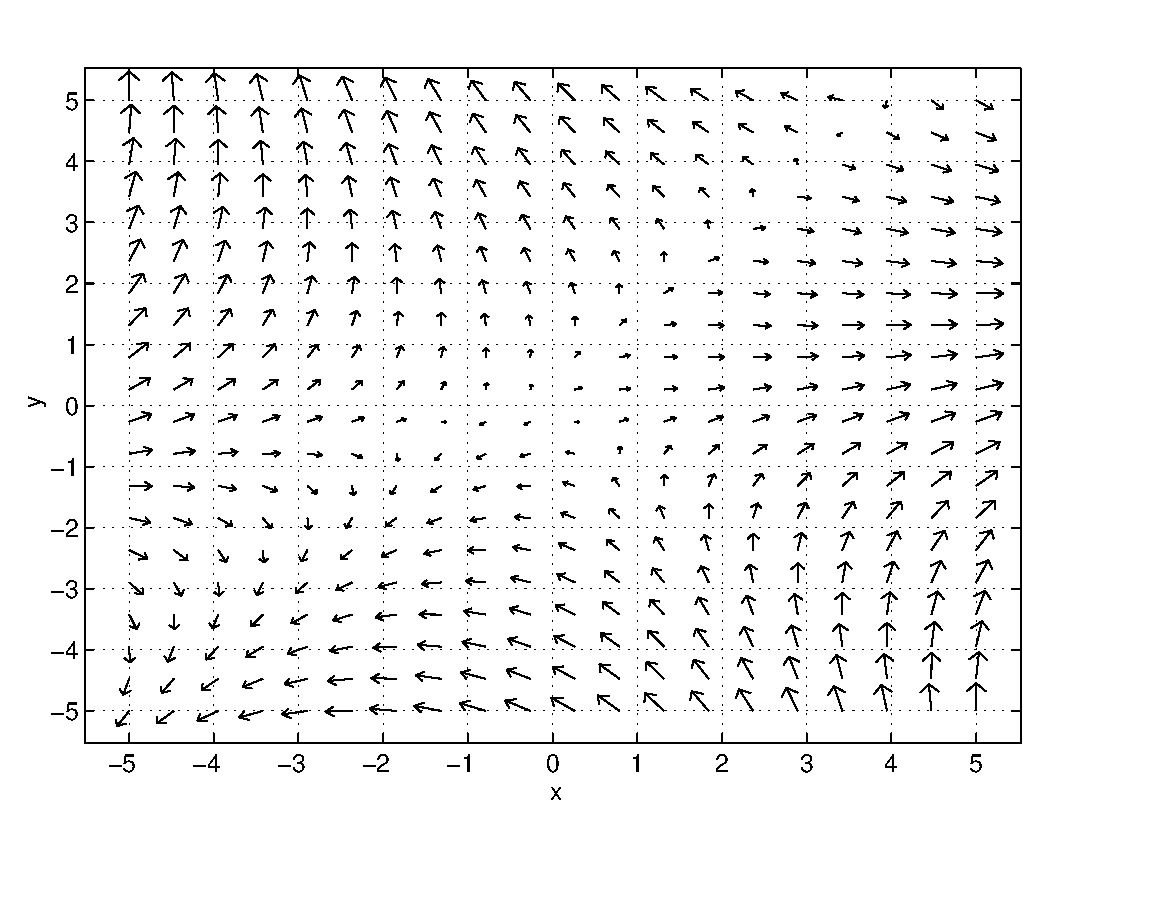
\psfig{file=../figures/saddlea.eps,width=3.2in}
           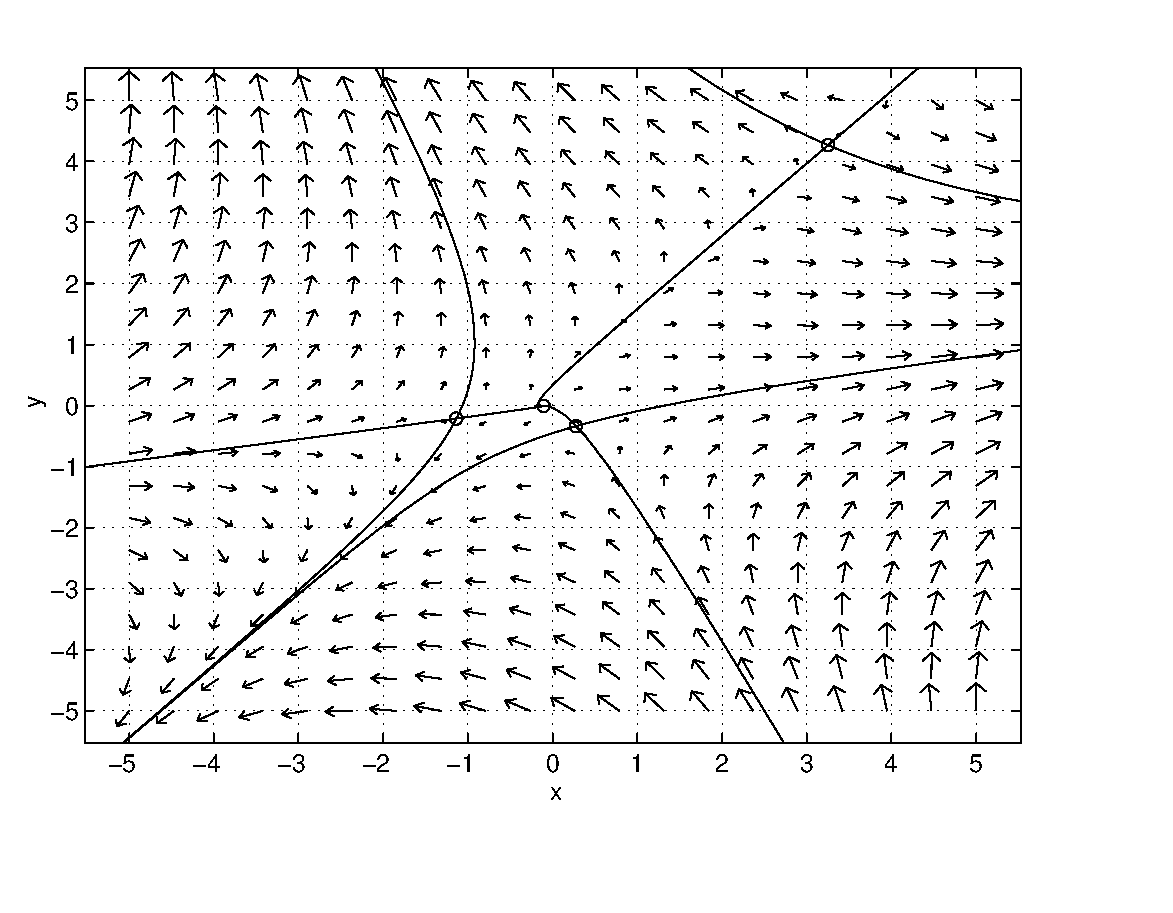
\psfig{file=../figures/saddleb.eps,width=3.2in}}
           \caption{(Left) Direction field of \protect\eqref{e:gradexam}.
	(Right) Phase plane with equilibria and stable orbits.}
           \label{F:gradexam}
\end{figure*}

\begin{figure}[htb]
           \centerline{%
           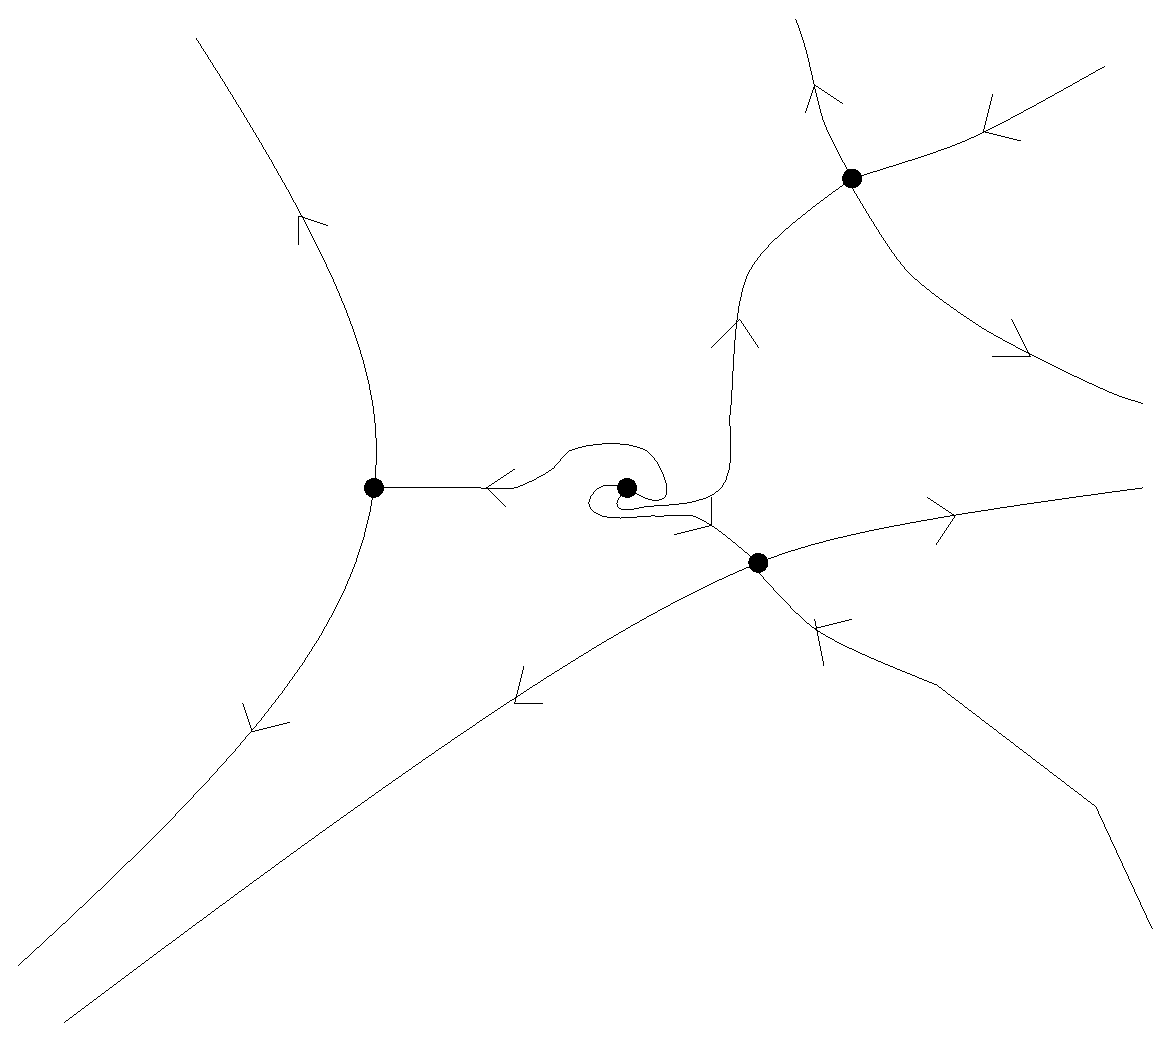
\psfig{file=../figures/grad.eps,width=3.in}}
           \caption{Stylized phase plane portrait of \protect\eqref{e:gradexam}.}
           \label{F:gradexamstyle}
\end{figure}

\EXER

\TEXER

\begin{exercise} \label{c8.2.1}
\begin{enumerate}
\item[(a)] Draw the phase line picture of the differential
equation 
\begin{equation}  \label{E:quad}
\frac{dx}{dt} = -x^2 +3x -2.
\end{equation}
\item[(b)] Let $x(t)$ be the solution to \eqref{E:quad} satisfying
$x(0)=-1$.  Determine $\dps\lim_{t\to\infty} x(t)$. 
\item[(c)] Let $y(t)$ be a solution to \eqref{E:quad} satisfying
$y(0)=0.5$. Sketch the time series of this solution.
\end{enumerate}

\begin{solution}

(a) \ans Figure~\ref{c8.2.1}a shows a phase line picture
of this system.

\soln There is a stable equilibrium at $x = 2$, and an unstable
equilibrium at $x = 1$, since $f(x) = -x^2 + 3x - 2 = (x - 1)(2 - x)$,
and since $f'(1) = 1 > 0$ and $f'(2) = -1 < 0$.

(b) \ans $\dps\lim_{t \to \infty} x(t) = -\infty$.

\soln The closest equilibrium to $x(0) = -1$ is $x = 1$, which is
unstable. 

(c) \ans Figure~\ref{c8.2.1}b shows the {\tt dfield5} graph of $y$.

\soln The trajectory of $y(t)$ with initial condition $y(0) = 0.5$ goes
to negative infinity in forward time, and limits on $y = 1$ in
backward time.

\begin{figure}[htb]
                       \centerline{%
                       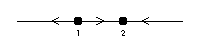
\psfig{file=exfigure/8-2-1a.eps,width=2.75in}
                       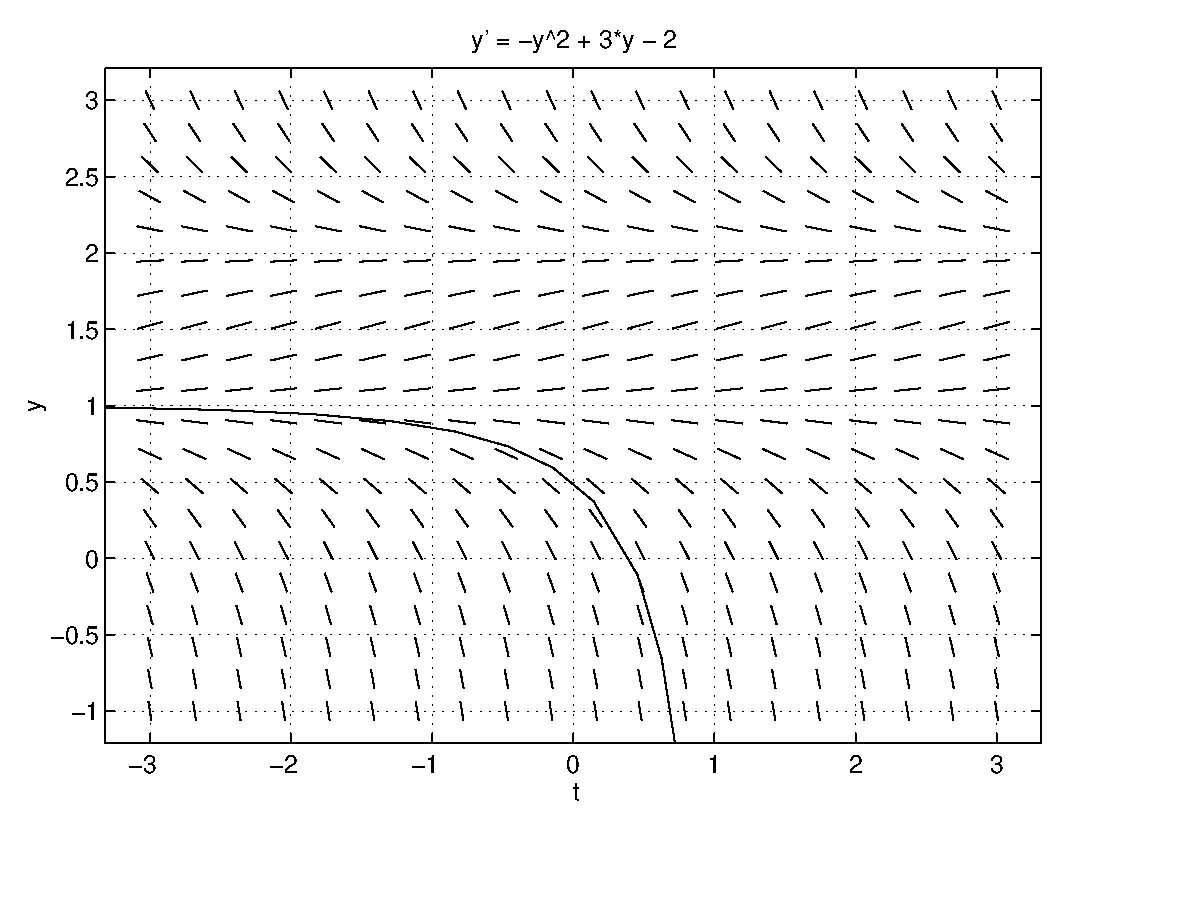
\psfig{file=exfigure/8-2-1b.eps,width=2.75in}}
                \exercaptwo{c8.2.1}
\end{figure}



\end{solution}
\end{exercise}

\begin{exercise} \label{E:popex}
Recall that the simplest population growth model
\index{population model} is 
\[
\frac{dp}{dt} = \lambda p,
\]
where $p(t)$ is the population at time $t$ and $\lambda$ is the
population growth rate. Suppose that the growth rate depends on
the size of the population, as follows:
\[
\lambda(p) = \lambda_0 - ap,
\]
where $\lambda_0>0$ and $a>0$ are constants.  Suppose that
$p(t)$ is a solution and $p(0)>0$.  What is the asymptotic
limit of the population in forward time, that is, what is
$\dps\lim_{t\to\infty} p(t)$?

\begin{solution}

\ans The asymptotic limit of the population in forward time is
$\frac{\lambda_0}{a}$.

\soln Substitute $\lambda(p)$ into the population model, obtaining
\[
\frac{dp}{dt} = (\lambda_0 - ap)p\equiv f(p).
\]
Solve for $f(p)= 0$ to find that the system has equilibria
at $p = 0$ and $p = \frac{\lambda_0}{a}$.  Then, find that
\[
\frac{df}{dp}(0) = \lambda_0 > 0 \AND
\frac{df}{dp}(\lambda_0/a) = -\lambda_0 < 0;
\]
so the equilibrium at $p = 0$ is unstable and the equilibrium at
$p = \frac{\lambda_0}{a} > 0$ is stable.  Therefore, a solution with 
initial population $p(0) > 0$ limits on $\frac{\lambda_0}{a}$.

\end{solution}
\end{exercise}  \index{population model}

\begin{exercise} \label{c8.2.3}
More generally, consider the population growth model
\begin{equation} \label{E:pop}
\frac{dp}{dt} = \lambda(p) p, 
\end{equation}
where the growth rate depends on the population.  Assume
\begin{enumerate}
\item[(i)] the growth rate is positive when the population is 
small, that is, $\lambda(0)>0$, and 
\item[(ii)] the growth rate decreases as the population
increases, that is, $\frac{d\lambda}{dp} < 0$ for all $p$.
\end{enumerate}
Consider the following:
\begin{enumerate}
\item[(a)] Show that equation \eqref{E:pop} has at most one
positive equilibrium $p_e>0$.
\item[(b)] Let $p(t)$ be a solution to \eqref{E:pop} with
$p(0)>0$. Determine the asymptotic limit of the population in
forward time, that is, determine $\dps\lim_{t\to\infty} p(t)$. 
\item[(c)] Relate your answer in (b) to the solution to
Exercise~\ref{E:popex}. 
\end{enumerate}
{\bf Hint:} There are two possible answers to (b) depending on
whether \eqref{E:pop} has one positive equilibrium or no positive 
equilibria.

\begin{solution}

(a) We are given $\frac{d\lambda}{dp} < 0$ for all $p$.  Thus $\lambda(p)$ is a 
monotonic decreasing function of $p$ when $p>0$ and the graph of 
$\lambda(p)$ can intersect $\lambda=0$ in at most one point.
Therefore, \eqref{E:pop} has at most one positive equilibrium.

(b) \ans If there exists a positive equilibrium $p_e$, then
$\dps\lim_{p \to \infty} p(t) = p_e$.  If no positive equilibrium
exists, then $\dps\lim_{p \to \infty} p(t) = \infty$.

\soln If there is a positive equilibrium, then it is asymptotically stable.
To verify this point differentiate the right hand side of \eqref{E:pop} with respect to 
$p$ and evaluate at $p=p_e$ obtaining
\[
\left.\frac{d}{dp}(\lambda(p)p)\right|_{p=p_e} = 
\lambda(p_e) + \lambda'(p_e)p_e = \lambda'(p_e)p_e <0
\]
since $\lambda(p_e) = 0$, $\lambda'(p_e) < 0$, and $p_e > 0$.  
So $p = p_e$ is a stable equilibrium, and the population limits on
$p_e$.

\para If no positive equilibrium exists, then $p = 0$, which is unstable,
is the only equilibrium, and the population grows without bound.

(c) Exercise~\ref{E:popex} is a specific example of \eqref{E:pop} in
which a positive equilibrium exists at $p = \frac{\lambda_0}{a}$.

\end{solution}
\end{exercise}

\noindent In Exercises~\ref{c8.2.4a} -- \ref{c8.2.4e} we review some
of the theory of planar linear systems of differential equations that
is needed in the study of planar nonlinear systems.  For the given 
matrix $C$, determine whether the origin is a hyperbolic equilibrium 
for the differential equation $\dot{X}=CX$.  When the origin is 
hyperbolic, what kind of system is it?
\begin{exercise} \label{c8.2.4a}
$C=\mattwo{0.1}{2}{-1}{-3}$. 

\begin{solution}
\ans The origin is a nodal sink.

\soln A matrix $C$ with nonzero trace and determinant is a hyperbolic
equilibrium.  In this case, $\trace(C) = -2.9$ and $\det(C) = 1.7$.
Since the determinant is positive and the trace is negative, the origin
is a sink. Since the discriminant is $1.61>0$ the origin is a node.

\end{solution}
\end{exercise}
\begin{exercise} \label{c8.2.4b}
$C=\mattwo{4}{-2}{1}{5}$. 

\begin{solution}
\ans The origin is a spiral source.

\soln In this case, $\trace(C) = 9$ and $\det(C) = 22$, so the origin
is a hyperbolic equilibrium and a source.  Since the discriminant is 
$-1<0$, the origin is a spiral.

\end{solution}
\end{exercise}
\begin{exercise} \label{c8.2.4c}
$C=\mattwo{2}{-1}{4}{-2}$. 

\begin{solution}
\ans The origin is not hyperbolic.

\soln Since $\trace(C) = 0$ and $\det(C) = 0$, the origin is not 
hyperbolic. 

\end{solution}
\end{exercise}
\begin{exercise} \label{c8.2.4d}
$C=\mattwo{1}{3}{-2}{-6}$.

\begin{solution}
\ans The origin is not hyperbolic.

\soln Since $\det(C) = 0$ the origin is not hyperbolic.

\end{solution}
\end{exercise}
\begin{exercise} \label{c8.2.4e}
$C=\mattwo{11}{-8}{18}{-13}$.

\begin{solution}
\ans The origin is an improper nodal sink.

\soln Since $\trace(C) = -2$ and $\det(C) = 1$, the equilibrium
is hyperbolic. Since the trace is negative, the origin is a sink.
Since the discriminant is $0$, the origin is an improper node. 

\end{solution}
\end{exercise}

\begin{exercise} \label{c8.2.5}
Consider the planar nonlinear system of ODEs
\begin{eqnarray*}
\frac{dx}{dt} & = & 1 - x - y \\
\frac{dy}{dt} & = & 2xy. 
\end{eqnarray*}
\begin{itemize}
\item[(a)] Find all equilibria of this system.
\item[(b)] Determine the behavior of trajectories in a small
neighborhood of each equilibrium.
\item[(c)] Sketch the phase portrait of this system.  {\bf Hint}: Check
for invariant axes.
\item[(d)] Use {\pplane} to verify your sketch.
\end{itemize}

\begin{solution}

(a) \ans The equilibria occur at $(x,y) = (1,0)$ and $(x,y) = (0,1)$.

\soln Solve $\frac{dx}{dt} = \frac{dy}{dt} = 0$.

(b) \ans The point $(x,y) = (1,0)$ is a saddle.  The point $(x,y) = (0,1)$
is a spiral sink.

\soln Let $f(x,y) = 1 - x - y$, $g(x,y) = 2xy$,
and $F = (f,g)$.  Then the Jacobian matrix is
\[
(dF)_{(x,y)} = \mattwo{f_x(x,y)}{f_y(x,y)}{g_x(x,y)}{g_y(x,y)}
= \mattwo{-1}{-1}{2y}{2x}.
\]
Specifically, at the equilibrium points:
\[
(dF)_{(1,0)} = \mattwo{-1}{-1}{0}{2} \qquad
(dF)_{(0,1)} = \mattwo{-1}{-1}{2}{0}.
\]
The eigenvalues of $(dF)_{(1,0)}$ are $\lambda_1 = 2$ and $\lambda_2 = -1$;
so the point is like a saddle in a small neighborhood.  The trace of
$(dF)_{(0,1)}$ is $-1 < 0$ and the determinant is $2 > 0$, so the
discriminant is negative and, within a small neighborhood, the point
is like a spiral sink.

(c) Compute the eigenvectors of the Jacobian of the saddle point $(1,0)$.
The invariant axes of $(1,0)$ are the eigendirections $(1,-3)$ and
$(1,0)$.  Use these vectors to graph the system.  Your sketch should
resemble the {\tt pplane5} graph in Figure~\ref{c8.2.5}.

\begin{figure}[htb]
                       \centerline{%
                       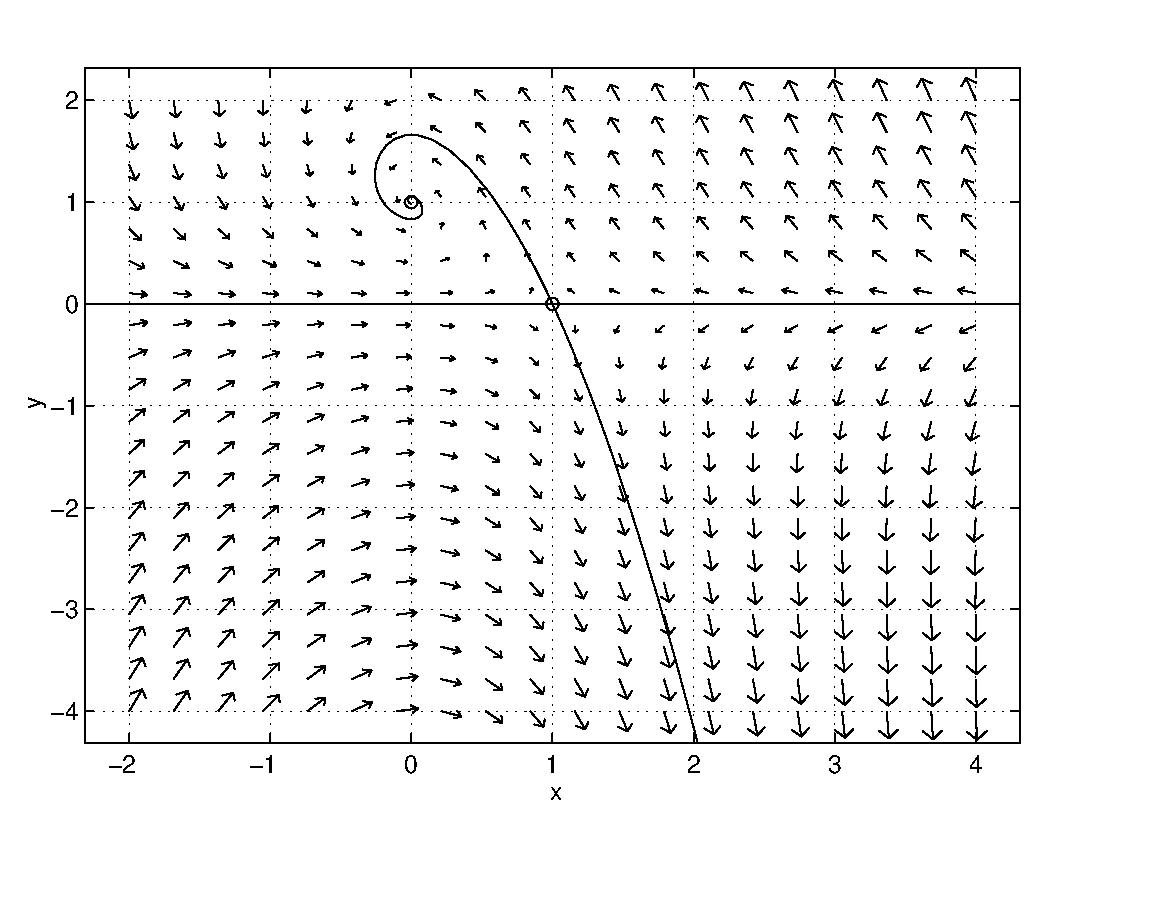
\psfig{file=exfigure/8-2-5.eps,width=3.0in}}
                \exercap{c8.2.5}
\end{figure}


\end{solution}
\end{exercise}

\begin{exercise} \label{c8.2.6}
Consider the planar nonlinear system of ODEs
\begin{eqnarray*}
\frac{dx}{dt} & = & 1 - 2x + y + x^2 - xy \\
\frac{dy}{dt} & = & y - y^2
\end{eqnarray*}
\begin{itemize}
\item[(a)] Find all equilibria of this system.
\item[(b)] Are the equilibria asymptotically stable or not?
\item[(c)] Determine the type of each equilibrium.
\end{itemize}

\begin{solution}

(a) \ans Equilibria occur at the points $(1,0)$, $(1,1)$, and $(2,1)$.

\soln Solve $0 = y - y^2$ to obtain $y = 1$ and $y = 0$, then substitute
these values for $y$ into $0 = 1 - 2x + y + x^2 - xy$ to find the points
at which $\frac{dx}{dt} = \frac{dy}{dt} = 0$.

(b) \ans The equilibria at $(1,0)$ and $(2,1)$ are not asymptotically
stable.  The equilibrium at $(1,1)$ is stable.

\soln Compute the Jacobian matrix of the system:
\[
(dJ)_{(x,y)} = \cmattwo{-2 + 2x - y}{1 - x}{0}{1 - 2y}
\]
Specifically, at the equilibrium points, the Jacobian matrices are
\[
(dJ)_{(1,0)} = \mattwo{0}{0}{0}{1} \qquad (dJ)_{(1,1)} =
\mattwo{-1}{0}{0}{-1} \qquad (dJ)_{(2,1)} = \mattwo{1}{-1}{0}{-1}.
\]
An equilibrium is asymptotically stable if both eigenvalues are
negative.  The eigenvalues of $(1,0)$ are $0$ and $1 > 0$.
The point $(1,1)$ has a double eigenvalue at $-1 < 0$.
The eigenvalues of $(1,1)$ are $-1 < 0$ and $1 > 0$.

(c) The equilibrium at $(1,0)$ is a saddle node, since the Jacobian
has one zero eigenvalue and one nonzero eigenvalue.  The equilibrium
at $(1,1)$ is a focus sink, since the Jacobian is a multiple of $I_2$
with negative real eigenvalue.  The equilibrium at $(2,1)$ is a
saddle point, since the Jacobian has one negative and one positive
eigenvalue.

\end{solution}
\end{exercise}

\begin{exercise} \label{c8.2.7}
Consider the system of differential equations \eqref{e:global2exam}
that depends on the constant $a$.  
\begin{itemize}
\item[(a)]	Find the equilibria of this system.
\item[(b)]	Find the Jacobian matrices at the equilibria.  
\item[(c)]	For which values of $a$ are the equilibria not
		hyperbolic?
\item[(d)]	For those values of $a$ where the equilibria are 
		hyperbolic, determine whether or not these equilibria 
		are asymptotically stable.
\item[(e)]	For each nonhyperbolic equilibrium, write the linearized 
		system and draw its phase plane.
\end{itemize}

\begin{solution}

(a) Solving system \eqref{e:global2exam} for $\dot{x} = \dot{y} = 0$
yields equilibria at $(0,0)$, $(\sqrt{2.2},0)$, and $(-\sqrt{2.2},0)$.

(b) The general Jacobian matrix for \eqref{e:global2exam} is
\[
(dJ)_{(x,y)} = \cmattwo{0}{1}{2.2 - 3x^2 + ay}{2.1 + ax}.
\]
The Jacobian matrices at the equilibria are:
\[ \begin{array}{rcl}
(dJ)_{(0,0)} & = & \cmattwo{0}{1}{2.2}{2.1} \\
(dJ)_{(\sqrt{2.2},0)} & = & \cmattwo{0}{1}{-4.4}{2.1 + \sqrt{2.2}a} \\
(dJ)_{(-\sqrt{2.2},0)} & = & \cmattwo{0}{1}{-4.4}{2.1 - \sqrt{2.2}a}. \\
\end{array}
\]

(c) \ans The Jacobian of the equilibrium at $(\sqrt{2.2},0)$ is not
hyperbolic at $a = -2.1\left/\sqrt{2.2}\right.$, and the Jacobian of the
equilibrium at $(-\sqrt{2.2},0)$ is not hyperbolic at
$a = 2.1\left/\sqrt{2.2}\right.$.

\soln Note that a matrix is nonhyperbolic if the determinant is positive
and the trace is zero.

(d) \ans The equilibrium at $(\sqrt{2.2},0)$ is asymptotically stable for
$a < -2.1\left/\sqrt{2.2}\right.$ and the equilibrium at
$(-\sqrt{2.2},0)$ is asymptotically stable for
$a > 2.1\left/\sqrt{2.2}\right.$.  Thus, there is no value of $a$ for which
both equilibria are stable.  The equilibrium at $(0,0)$ is not stable,
since the eigenvalues of the Jacobian have opposite sign.

\soln Note that the determinant of the Jacobian is always positive, so
the equilibria are stable for values of $a$ at which the trace is negative.

(e) For $a = -2.1/\sqrt{2.2}$, the equilibrium at $(\sqrt{2.2},0)$
is non-hyperbolic, with Jacobian matrix
\[
(dJ)_{(\sqrt{2.2},0)} = \mattwo{0}{1}{-4.4}{0}.
\]
The linear system $\dot{X} = (dJ)_{(\sqrt{2.2},0)}X$ is pictured in
Figure~\ref{c8.2.7}.  Note that the system is a center.  For
$a = 2.1/\sqrt{2.2}$, the equilibrium at $(-\sqrt{2.2},0)$ is
nonhyperbolic.  Its Jacobian at this point is identical to
$(dJ)_{(\sqrt{2.2},0)}$.

\begin{figure}[htb]
                       \centerline{%
                       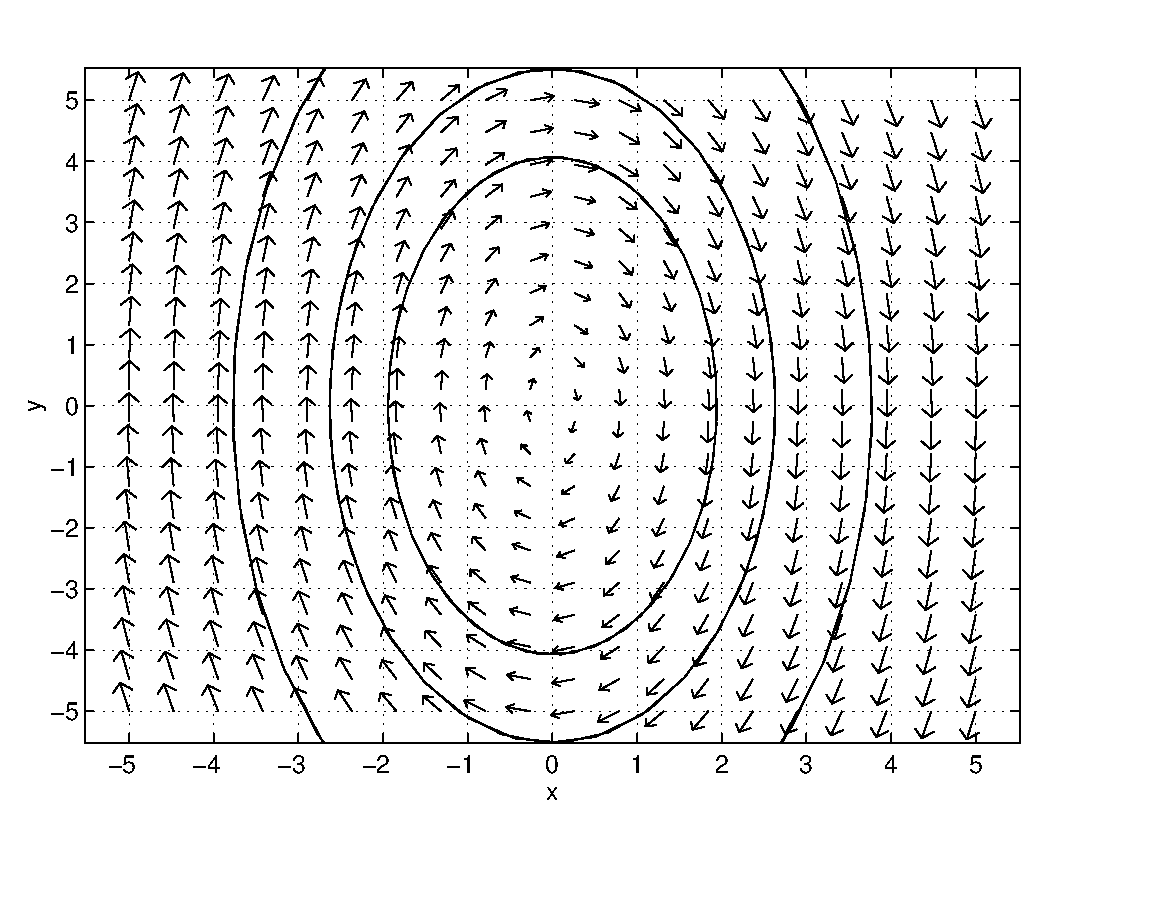
\psfig{file=exfigure/8-2-7.eps,width=3.0in}}
                \exercap{c8.2.7}
\end{figure}

\end{solution}
\end{exercise}

\begin{exercise} \label{c8.2.8}
Find all equilibria of the system of ODEs
\begin{eqnarray*}
\dot{x} & = & 2x - y \\
\dot{y} & = & 11x + x^2 - 3y^2.
\end{eqnarray*}
Also determine the types of each of these equilibria.

\begin{solution}

\ans There are two equilibria: a spiral source at $(0,0)$, and a saddle
at $(1,2)$.

\soln Solve the system for $\dot{x} = \dot{y} = 0$.  Then, compute the
Jacobian matrices at the equilibria, in this case
\[
(dJ)_{(0,0)} = \mattwo{2}{-1}{11}{0} \qquad
(dJ)_{(1,2)} = \mattwo{2}{-1}{13}{-12}
\]
and compute the eigenvalues of these matrices.  The eigenvalues of the
Jacobian of $(0,0)$ are $1 \pm \sqrt{10}i$.  Since the eigenvalues
are complex with positive real part, the equilibrium is
a spiral source.  The determinant of the Jacobian of $(1,2)$ is
$-11 < 0$.  Thus the equilibrium is a saddle.

\end{solution}
\end{exercise}

\begin{exercise}  \label{E:nonhyp}
\noindent (a)  Show that the origin is the only equilibrium of 
\begin{matlabEquation}  \label{e:nonhypcenter}
\begin{array}{rcl}
\dot{x} & = & y -x^3 -2xy^2 \\
\dot{y} & = & -x - y^3
\end{array}
\end{matlabEquation}
and that the linearized system about the origin is a 
center\index{center}. Hence the origin is not hyperbolic.

\noindent (b)  Let $r=\sqrt{x^2+y^2}$ be the distance of $(x,y)$ from the 
origin.  Let $(x(t),y(t))$ be a solution to \eqref{e:nonhypcenter} and show 
that $r(t)$ satisfies the differential equation
\[
\dot{r}(t) = -r(t)^3
\]
Use this fact to show that the origin is an asymptotically stable equilibrium
of \eqref{e:nonhypcenter}.  (Hence the phase portraits of the linearized and 
nonlinear systems are different on all neighborhoods of the origin and  
the hyperbolicity assumption in Theorem~\ref{T:linearization} is needed.)

\begin{solution}

(a) Find all equilibria by computing $x$ and $y$ for $\dot{x} =
\dot{y} = 0$.  Then, from the second equation, $x = -y^3$, so
substituting into the first equation yields
\[
0 = y^9 + 2y^5 + y = y(y^4 + 1)^2.
\]
The only solution to this equation over the complex number system is
$y = 0$.  Therefore, the origin is the only equilibrium of
\eqref{e:nonhypcenter}.  The Jacobian matrix of \eqref{e:nonhypcenter} at
the origin is 
\[
(dJ)_{(0,0)} = \mattwo{0}{1}{-1}{0}.
\]
The eigenvalues of this Jacobian are $\pm i$.  Therefore, the equilibrium
is a center.

(b) First, compute $\dot{r}$:
\[
\frac{d}{dt}(r) = \frac{d}{dt}(\sqrt{x^2 + y^2}) =
\frac{1}{2\sqrt{x^2 + y^2}}\left(\frac{d}{dt}(x^2 + y^2)\right)
= \frac{1}{r}(x\dot{x} + y\dot{y}).
\]
Then, substitute \eqref{e:nonhypcenter} to obtain
\[
\dot{r} = \frac{1}{r}(x(y - x^3 - 2xy^2) + y(-x - y^3))
= -\frac{1}{r}(x^2 + y^2)^2 = -r^3.
\]
Note that $r''(t) = -3r(t)^2 < 0$.  Thus, $r = 0$ is a stable equilibrium
of \eqref{e:nonhypcenter}.

\end{solution}
\end{exercise}

\CEXER

\begin{exercise} \label{c8.2.10}
Use {\pplane} to determine the phase portraits of the nonlinear system
\eqref{e:nonhypcenter}.  Verify that {\pplane} finds (approximately) 
periodic solutions on sufficiently small neighborhoods of the origin.  This 
experiment, coupled with the results from Exercise~\ref{E:nonhyp}, suggests 
that the numerical methods employed by {\pplane} fail sufficiently close 
to nonhyperbolic equilibria.

\begin{solution}

System \eqref{e:nonhypcenter} is shown in Figure~\ref{c8.2.10}a with four
trajectories.  Figure~\ref{c8.2.10}b shows the system in a small
neighborhood of the origin.  In this graph, trajectories appear to be
closed orbits.  Using the {\tt find an equilibrium} command, we find
that \Matlab considers the origin to be a spiral.

\begin{figure}[htb]
                       \centerline{%
                       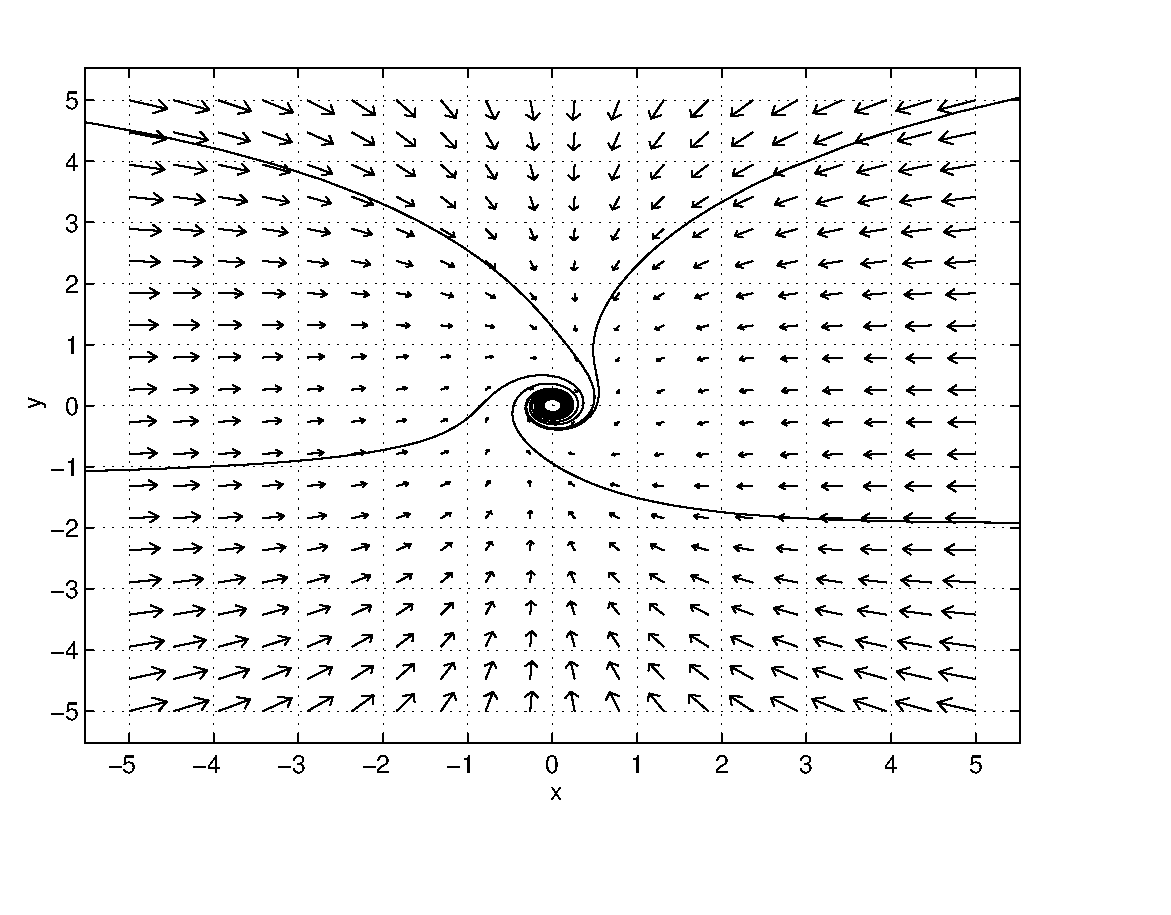
\psfig{file=exfigure/8-2-10a.eps,width=2.75in}
                       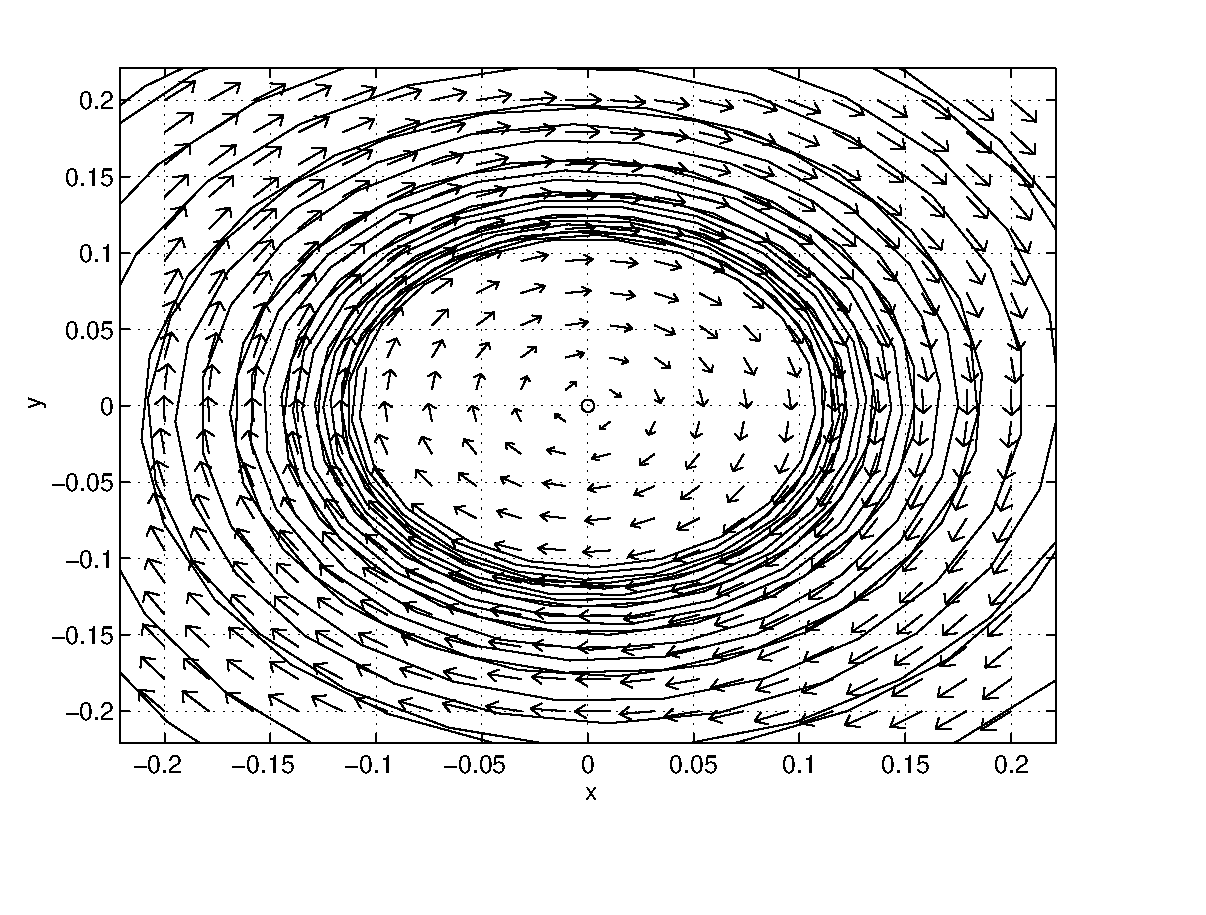
\psfig{file=exfigure/8-2-10b.eps,width=2.75in}}
                \exercaptwo{c8.2.10}
\end{figure}

\end{solution}
\end{exercise}

\begin{exercise} \label{c8.2.11}
Consider the system of differential equations 
\begin{matlabEquation}\label{MATLAB:6}
\begin{array}{rcl}
\dot{x} & = & -x - y + x^2 - y^2\\
\dot{y} & = & 0.25x - 3y - 2xy + y^2
\end{array}
\end{matlabEquation}
\begin{itemize}
\item[(a)] Use {\pplane} to verify that the origin is a nodal
sink\index{nodal sink} with 
eigenvalues $\lambda_1=-2.866$ and $\lambda_2=-1.134$.
\item[(b)] Use {\pplane} on the square $-1\leq x,y \leq 1$ to 
verify that trajectories starting near the origin approach the 
origin on curves tangent to the eigendirection\index{eigendirection} 
corresponding to the eigenvalue $\lambda_2$.
\end{itemize}

\begin{solution}

(a) The {\tt pplane5} command {\tt find an equilibrium} verifies this.

(b) {\tt pplane5} computes the eigenvectors as $v_1 = (0.4723,0.8814)$
(the eigenvector associated to $\lambda_1$) and $v_2 =
(0.9911,0.1328)$ (the eigenvector associated to $\lambda_2$).
Indeed, trajectories approach the origin in the direction of $v_2$.

\end{solution}
\end{exercise}

\begin{exercise} \label{c8.2.12}
Using {\pplane}, find all equilibria of 
\begin{matlabEquation}\label{MATLAB:7}
\begin{array}{rcl}
\dot{x} & = & 3x-2y-3x^2+y^2 \\
\dot{y} & = & -x+y-3xy
\end{array}
\end{matlabEquation}
on the square $-2\leq x,y \leq 2$.  Determine the type of 
equilibria and draw a phase portrait for this system of equations. 

\begin{solution}

By evaluation using {\tt pplane5}, the equilibria on the square
$-2 \leq x,y \leq 2$ are: a nodal source at $(0,0)$, a saddle point
at $(0.1041, 0.1513)$, a spiral source at $(0.2768,1.632)$, and a
spiral sink at $(1.286,-0.45)$.  Figure~\ref{c8.2.12} shows
equilibria and sample trajectories of the system.

\begin{figure}[htb]
                       \centerline{%
                       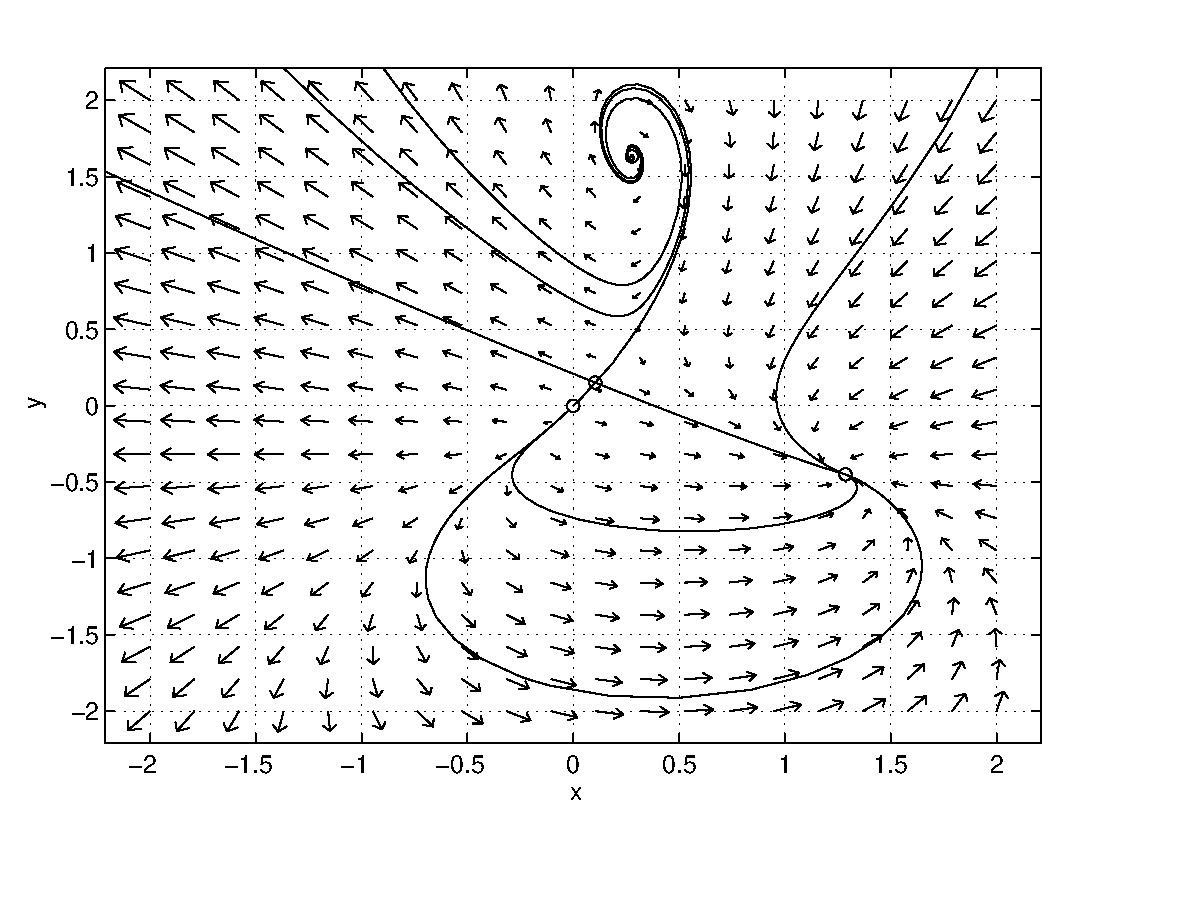
\psfig{file=exfigure/8-2-12.eps,width=3.0in}}
                \exercap{c8.2.12}
\end{figure}


\end{solution}
\end{exercise}

\end{document}
